% !TeX root =../main.tex

\chapter{Results and Discussion}
\label{sec:cha4}
Having laid the foundation for an LTspice inductor model and explained the limits of the inbuilt hysteresis model, the simulated inductor is now compared to a physical inductor. First, a setup to measure the voltages and currents of a synchronous buck converter is presented in section \ref{sec:buck_converter_measurement}. Its resulting measurements are assessed for expected behaviour, removing measurement errors. The setup is then used in section \ref{sec:validation_of_the_inductor_saturation_model} to validate the saturation model created in section \ref{sec:saturation_behaviour_of_the_inductor} by comparing the ripple current behaviour for different currents through the inductor. Combining the results in section \ref{sec:complete_simulation_of_the_buck_converter}, a complete synchronous buck converter is recreated in LTspice, by incorporating the provided \ac{GaNFET} models. The simulated losses are then compared to the measured losses and an approach to estimate the ideal switching frequency is proposed in section \ref{sec:evaluation}. 

\section{Buck Converter Measurement}\label{sec:buck_converter_measurement}
To compare the simulation to real-world measurements, multiple buck converters are built and measured. First, the parts, equipment and settings used for the physical measurements are discussed. After that, the results of the measurements are presented and evaluated based on the theory introduced in chapter \ref{sec:fundamentals}.
\subsection{Setup of the Buck Converter Measurement}\label{sec:setup_of_the_buck_converter}
For the validation and comparison of simulation and physical measurements, four buck converters with interchangeable inductors were built. As a base, each individual buck converter consists of a \ac{GaNFET} half-bridge development board, provided by the manufacturer EPC and chosen because of their provided \ac{GaNFET} LTspice model. The used \acp{GaNFET} are:
\begin{table}[H]
    \centering
    \caption{List of used \acp{GaNFET} and  their associated development boards}
    \begin{tabular}{|r|c|c|c|c|}
        \hline
        \ac{GaNFET} & EPC2308 & EPC2307 & EPC2088 & EPC2305 \\
        \hline
        Development Board & EPC90148 & EPC90150 & EPC90154 & EPC90143\\
        \hline
    \end{tabular}
    \label{tab:list_of_GaNFETs}
\end{table}
Each development board comes with two \acp{GaNFET}, controlled by an input \ac{PWM} signal. The signal directly dictates the behaviour of the \ac{HS} \ac{GaNFET}, while the \ac{LS} \ac{GaNFET} is controlled by a chip, which inverts the signal and adds a pre-set dead time. The dead time is adjustable but left at the default \SI{10}{\nano\s}. Onto the development board, a DuPont connector is soldered, which enables the easy swapping of the five different inductors, listed in \ref{tab:list_of_inductors}. Lastly, a \SI{47}{\micro\F} capacitor is soldered to the output. Connected to the development board are two power supplies, a frequency generator and an electronic load. The first power supply delivers a constant \SI{30}{\V} input voltage, verified at the drain of the \ac{HS} \ac{GaNFET}. Supplying the gate drivers, \ac{PWM} inverting logic and the dead time logic is a second power supply, set to \SI{11}{\V}. The power output by it does not factor into the efficiency measurements of the buck converter. Thirdly, the \ac{PWM} signal is generated by the frequency generator with an \SI{5}{\V} amplitude and a 50\% duty cycle. Lastly, the electronic load is connected to the buck converter's output, drawing a constant \SI{2}{\A} output current.\\
For each inductor, a separate circuit board is created with a wire loop, allowing the current and voltage across the inductor to be measured. The back side of the circuit board connects to the DuPont connector on the development board, enabling quick interchanges of the used inductors.
Using an oscilloscope the individual currents into and out of the buck converter as well as the current through the inductor are measured with current clamps. The voltages at the drain and source of the \ac{HS} \ac{GaNFET} and the voltages before and after the inductor are also measured while using the output of the \ac{PWM} source to trigger the measurement. These measurements are then combined, to give the power fed into the buck converter, going out to the load and lost by the inductor. 
\begin{figure}[H]
    \begin{subfigure}[b]{0.50\textwidth}
        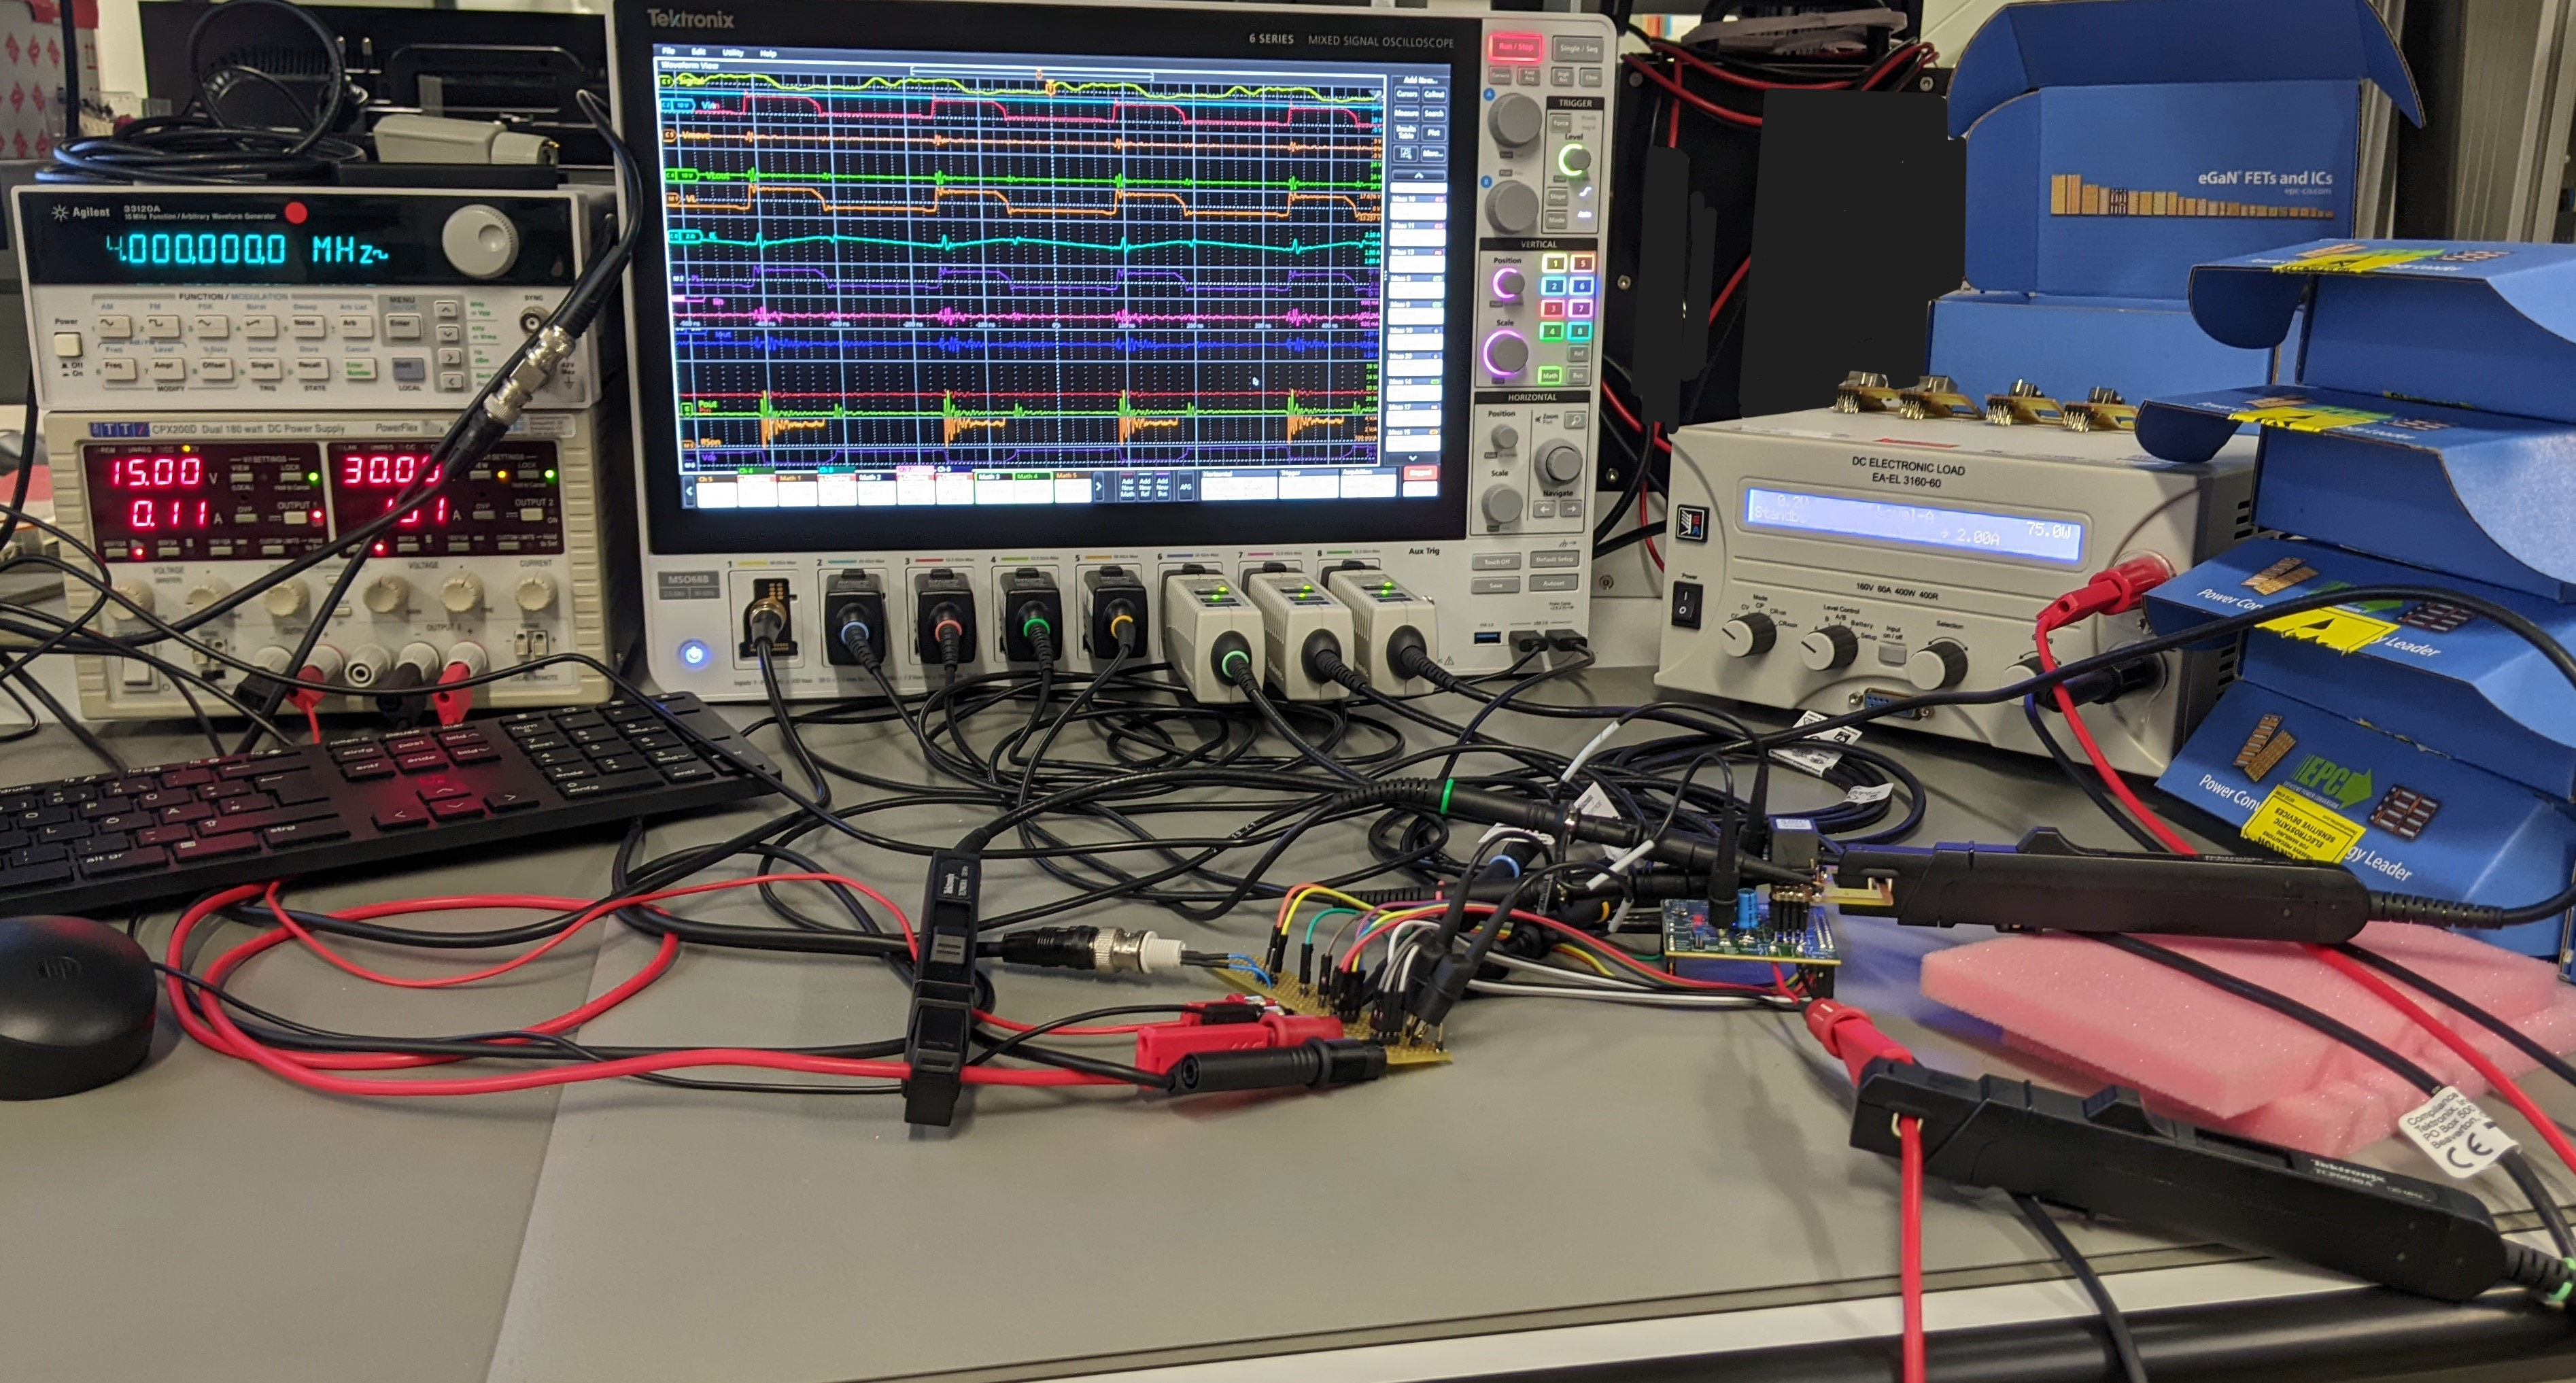
\includegraphics[width=\textwidth]{Bilder/Kapitel4/Measurement_Work_Station_cropped.jpg}
        \caption{Measurement equipment}
    \end{subfigure}
    \begin{subfigure}[b]{0.50\textwidth}
        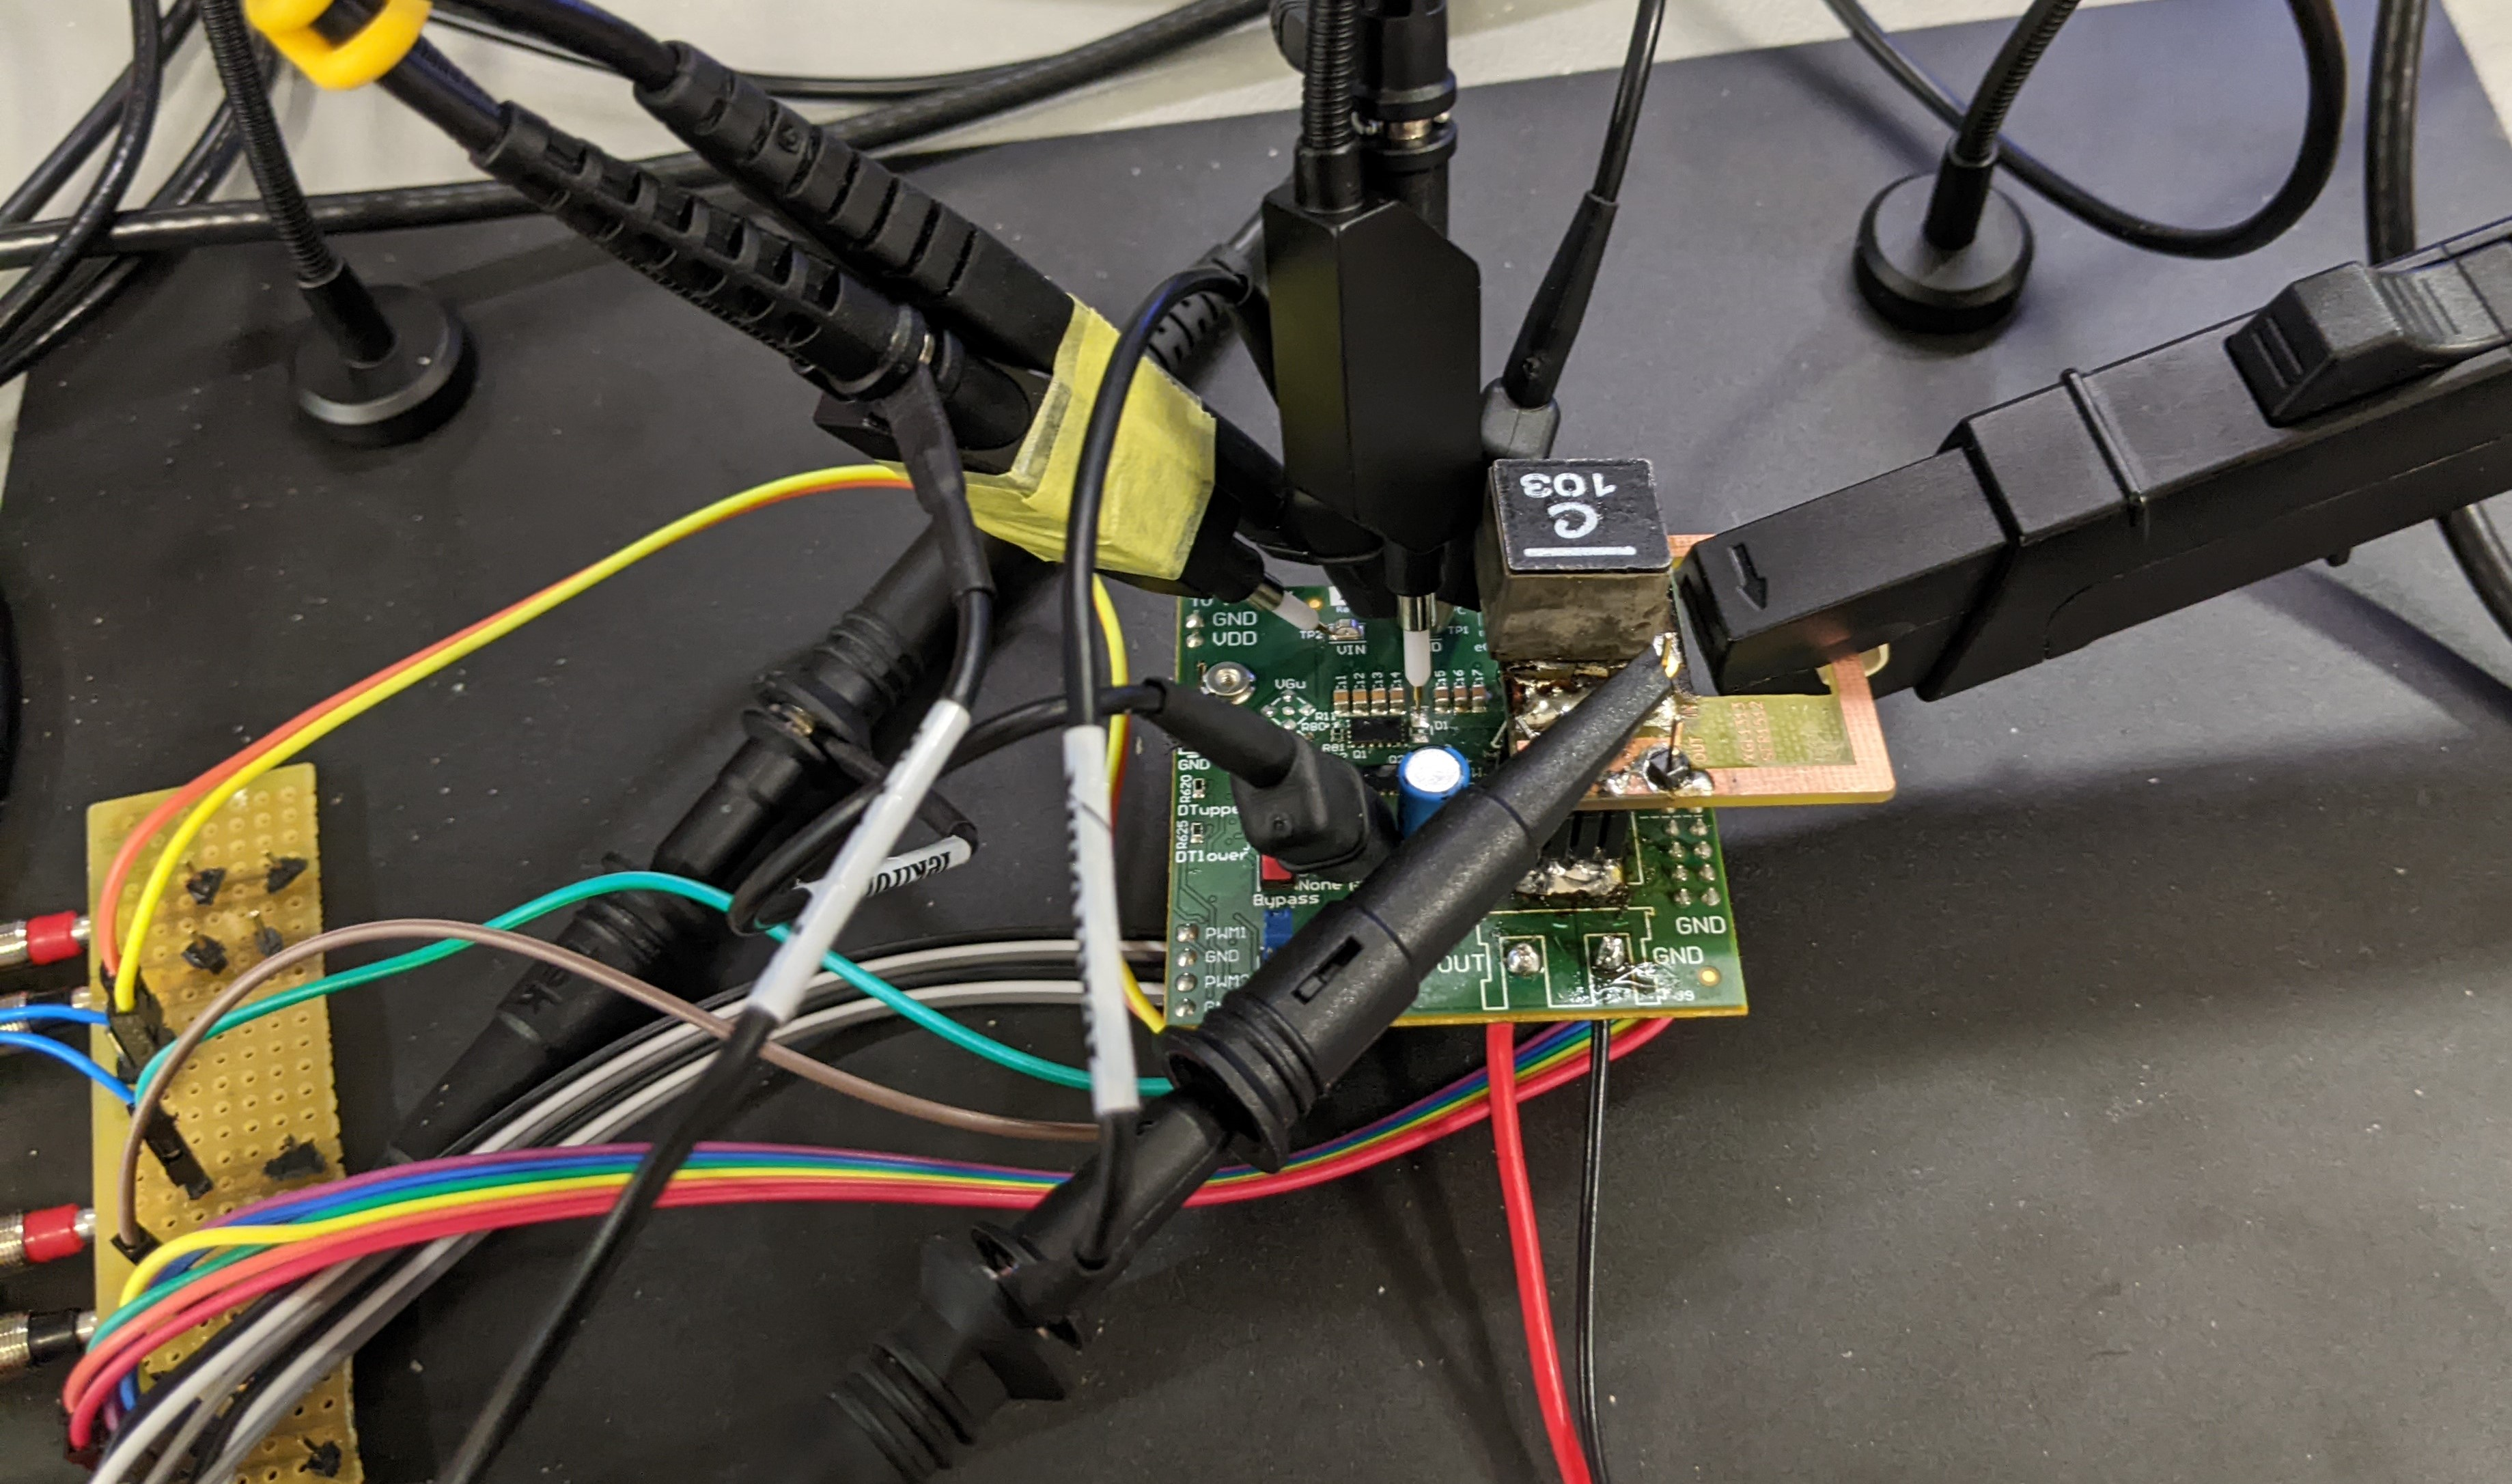
\includegraphics[width=\textwidth]{Bilder/Kapitel4/Measurement_Work_Station_close_cropped.jpg}
        \caption{Closeup of the buck converter}
    \end{subfigure}
    \caption{Measurement Setup}
    \label{fig:hysteresis_comparison}							
\end{figure}
The range of the switching frequency with which the buck converter can be controlled is limited by two factors. On the low end of the frequency spectrum, the ripple current amplitude increases exponentially. Because of this, the lowest analysed switching frequency is set to \SI{80}{\kilo\Hz}, avoiding saturation of the inductor. On the high end, the switching frequency is limited by the ability of the \ac{PWM} source. At over \SI{4}{\mega\Hz} the noise in the switching \ac{PWM} signal is too great to guarantee the reliant operation of the buck converter. Thus these two frequencies define the boundaries of the observed switching frequency range. By random probing of the buck converter for different frequencies, the semi-optimum switching frequency of the different setups turned out to always be at the lower end of this spectrum. Because of this the measured frequencies have a bias towards the kilohertz range and do not increase linearly. Five further frequencies were chosen to measure the behaviour of the buck converter, totalling the following seven measured frequencies: \SI{80}{\kilo\Hz}, \SI{100}{\kilo\Hz}, \SI{300}{\kilo\Hz}, \SI{800}{\kilo\Hz}, \SI{1}{\mega\Hz}, \SI{2}{\mega\Hz} and \SI{4}{\mega\Hz}.

\subsection{Measuring the Buck Converter}\label{sec:measuring_the_buck_converter}
Measuring the buck converter is done 20 times, once for each possible combination of inductor and \ac{GaNFET}. The input voltage is checked every measurement to ensure a constant \SI{30}{V} supply to the \ac{HS} \ac{GaNFET}, as other circuitry on the development board influences this voltage. By doing so the comparison to the simulation can be made more easily.\\
Dividing the output power by the input power yields the efficiency of the buck converter. Here the efficiency of the buck converter for the different \acp{GaNFET} using the \textit{XGL1313-223ME} inductor is displayed.
\begin{figure}[H]
    \centering
    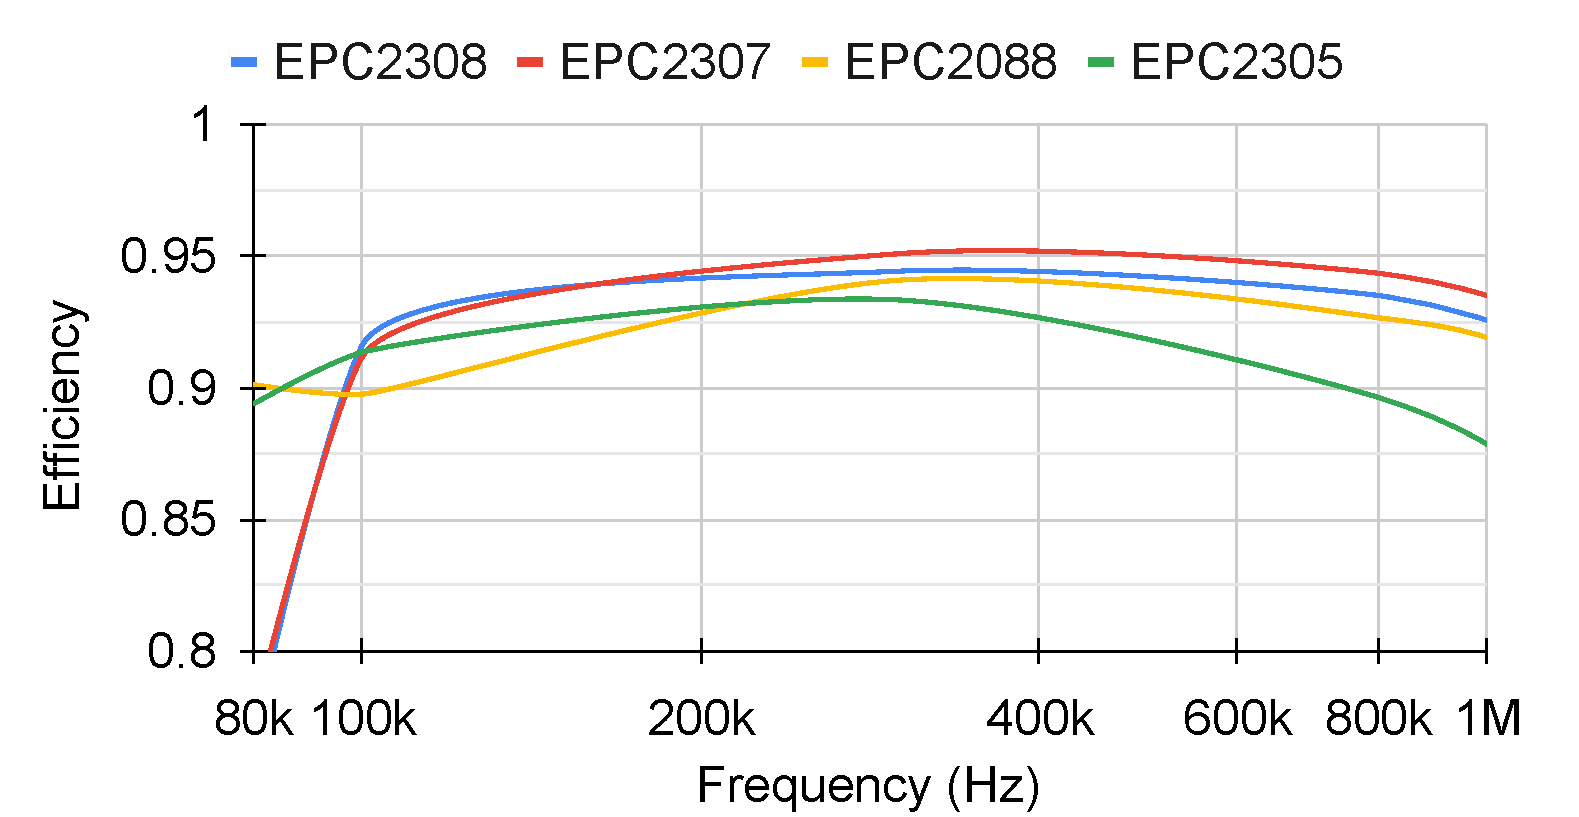
\includegraphics[width=0.75\linewidth]{Bilder//Kapitel4/BC_Meas_Efficiency_GaN_XGL103.pdf}
    \caption{Efficiency of the buck converter for different \acp{GaNFET} using the \textit{XGL1313-223ME} inductor}
    \label{fig:efficiency_bc_GaNFETs}
\end{figure}
For two \acp{GaNFET}, there is a great gain in efficiency between \SI{80}{\kilo\Hz} and \SI{100}{\kilo\Hz}, while for the other two \acp{GaNFET} the efficiency only changes minimally. Since the inductor is the same for all dour measurements, the difference in efficiency between the \acp{GaNFET} can only be caused by them. However, no source of power loss in the \acp{GaNFET} discussed in chapter \ref{sec:losses_in_switching_elements}, could cause such a drastic change in efficiency. Furthermore, as with low frequencies the ripple current of the inductor increases, it should dominate the loss behaviour. The conclusion therefore links this phenomenon to the rest of the development board. Due to this, these first measurements are not taken into consideration.\\
Comparing the efficiency for the different inductors while using the \textit{EPC2088} qualitatively shows the frequency-dependent behaviour of the losses. 
\begin{figure}[H]
    \centering
    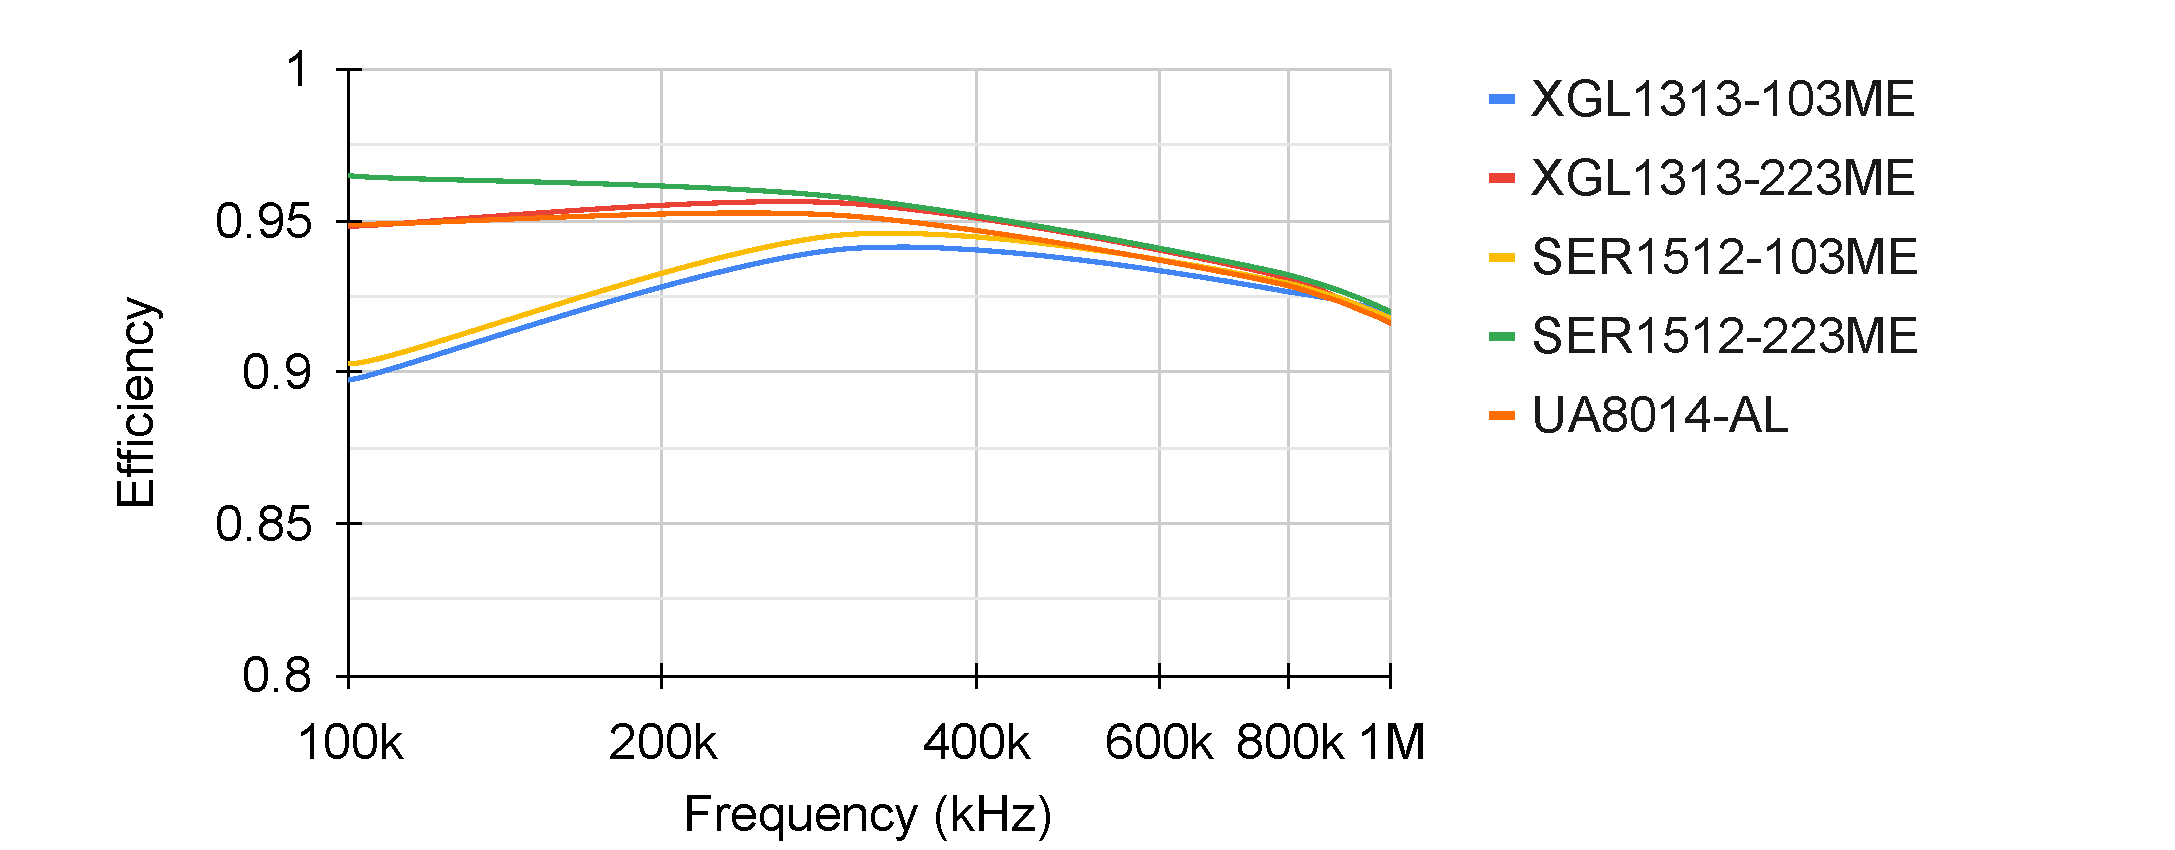
\includegraphics[width=0.95\linewidth]{Bilder//Kapitel4/BC_Meas_Efficiency_Inductor_EPC2088.pdf}
    \caption{Efficiency of the buck converter for different inductors using the \textit{EPC2088} \acp{GaNFET}}
    \label{fig:efficiency_bc_inductors}
\end{figure}
The graph can be split into two segments. For high frequencies, the losses are close to independent of the inductor and are mainly determined by the \acp{GaNFET}, as shown by the divergence of the lines in figure \ref{fig:efficiency_bc_GaNFETs} for higher frequencies. For low frequencies on the other hand, the inductors are the main cause of losses. This is shown in figure \ref{fig:efficiency_bc_inductors}, as changing the inductor has an effect on the efficiency for low frequencies but only barely influences the efficiency at high frequencies. As inductor losses are heavily influenced by the amplitude of the ripple current, inductors with a higher inductance are more efficient at these frequencies. In figure \ref{fig:efficiency_bc_inductors}, inductors with a similar inductance behave alike. The point with the highest efficiency is in the middle between these two regions, where the combined losses are minimal.\\

Visualising the loss behaviour of the \textit{XGL1313-103ME} inductor and the \textit{EPC2088} \acp{GaNFET} shows the linear high-frequency behaviour of the \acp{GaNFET} losses. 
\begin{figure}[H]
        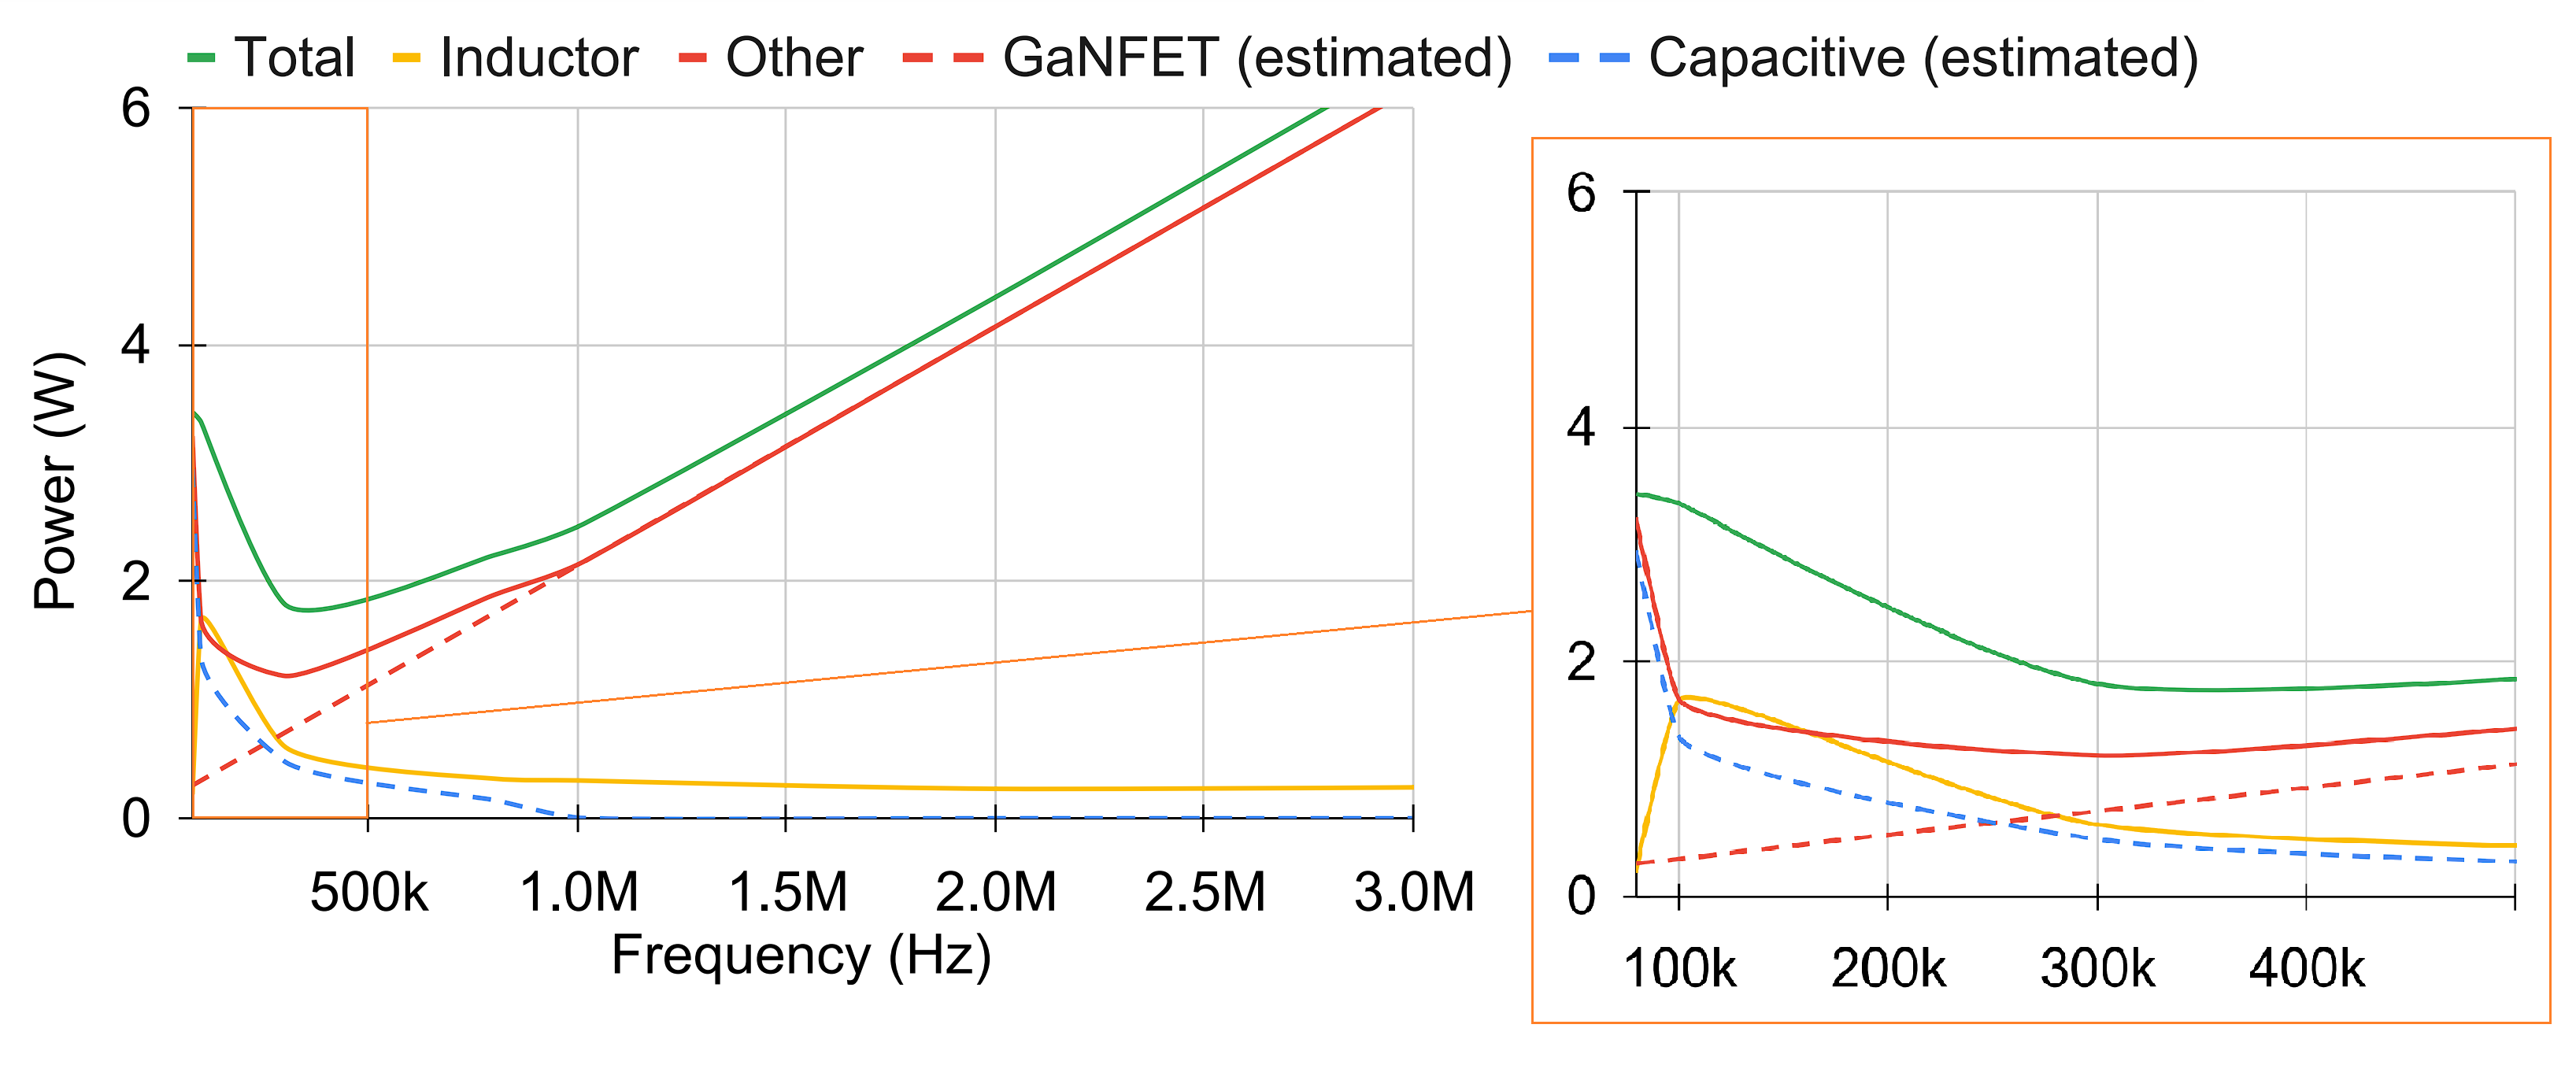
\includegraphics[width=1\textwidth]{Bilder/Kapitel4/BC_Meas_Losses_in_XGL103.png}
        \caption{Frequency dependant loss in the buck converter using the \textit{XGL1313-103ME} inductor and the \textit{EPC2088} \ac{GaNFET}}
        \label{fig:bc_losses_measured}							
\end{figure}
This is expected, as these losses mainly arise from switching losses, which are proportional to frequency. Also, a decrease in the inductor losses is visible, explained by the higher frequency reducing the size of the ripple current amplitude. \\
%The jump in inductor losses between \SI{800}{\kilo\Hz} and \SI{1}{\mega\Hz}, is an artifact created by the equipment used. The artefact appears in all measurements at exactly this change in frequency and might be caused by a mode switch in the electronic load, adjusting for the higher frequency ripply current it experiences. 
Regarding the not mentioned combinations of inductors and \acp{GaNFET}, their behaviour follows that of the chosen example and their optimal frequency lies between \SI{100}{\kilo\Hz} and \SI{300}{\kilo\Hz}. 

\section{Validation of the Inductor Saturation Model}\label{sec:validation_of_the_inductor_saturation_model}
To test the viability of the saturation model created in chapter \ref{sec:saturation_behaviour_of_the_inductor}, the output current of the buck converter is increased beyond the saturation current up to \SI{20}{A}. As this forces the inductor into saturation, the inductance decreases and the ripple current increases as a result. 
\subsection{Inductor Saturation Simulation and Measurement Setup}
Simulating the inductor is done by combining the inductor-\ac{ECM} together with the inductance defined by the \textit{flux}-function. The new \ac{ECM} is then connected to a pulsing voltage source and constant current load. The voltage source simulates the excitation caused by the switching elements, without using direct \ac{GaNFET} models. This ensures that all effects are purely based on the inductor. To enable a ripple current to flow, a capacitor is also added in parallel to the current source, completing the circuit diagram shown here.
\begin{figure}[H]
    \centering
    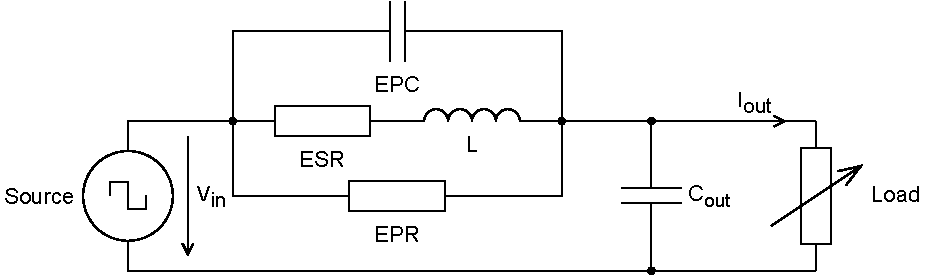
\includegraphics[width=1\linewidth]{Bilder/Kapitel4/Saturation_Validation_ECM.pdf}
    \caption{Circuit Diagram simulating the behaviour of a buck converter}
    \label{fig:saturation_validation_circuit_diagramm}
\end{figure}
The voltage source sends out rectangular voltage pulses with a 50\% duty cycle, \SI{30}{\V} peek at a switching frequency of \SI{300}{\kilo\Hz}. Measuring the peek-to-peek amplitude of the ripple current flowing through the \ac{ECM}, the current drawn by the simulated load is increased step by step from \SI{0.5}{\A} to \SI{20}{\A}. This process is then repeated for all five inductors.\\
Similarly for the physical measurement, the buck converter is set to the same settings and uses the setup described in section \ref{sec:setup_of_the_buck_converter}. Choosing \textit{EPC2308} as the switching element, results in a high efficiency of the buck converter, minimizing the distortion of the measurements. 
\subsection{Comparison of the Simulated and Measured Saturation Behaviour}
Observing the measured data, an \ac{DC} dependent increase of the ripple currents amplitude is detected for all inductors. This increase, however, is not uniform between the inductors. For the \textit{SER1512} inductors, their ripple current scales up drastically, as soon as the approximate saturation current of \SI{7}{\A} and \SI{10}{\A} is reached. At \SI{20}{\A} \ac{DC} both register a peek-to-peek ripple current amplitude of more than \SI{15}{\A}. In comparison, the \textit{XGL1313} inductors only increase their ripple current amplitude slightly after reaching saturation. Furthermore, the \textit{UA8014-AL} inductor's ripple current amplitude first increases quickly after reaching saturation but then slows down.
\begin{figure}[H]
    \centering
    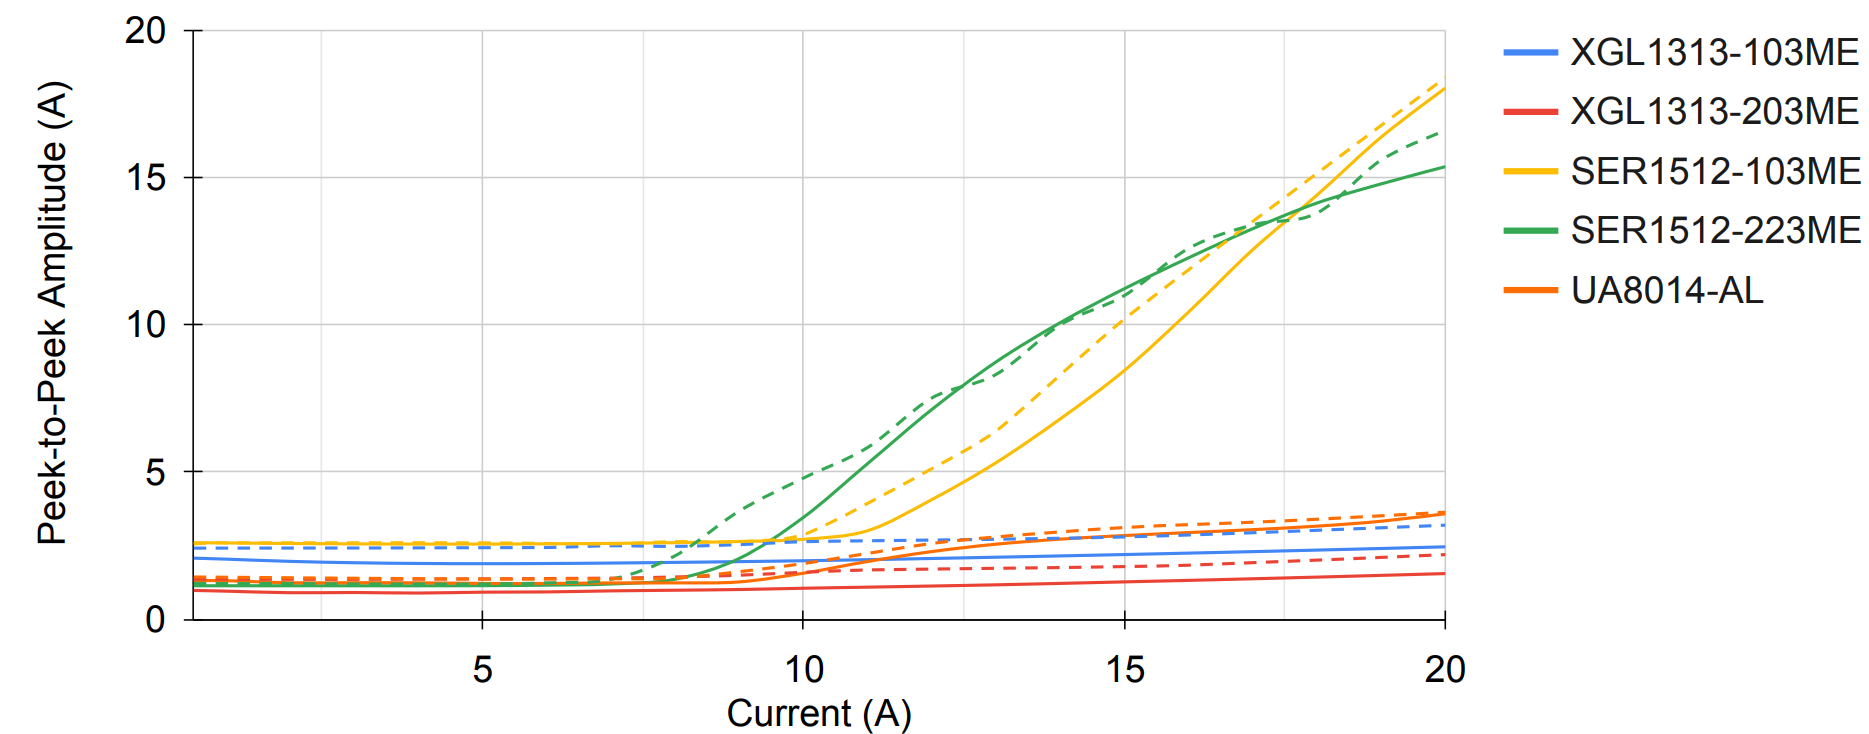
\includegraphics[width=1\linewidth]{Bilder//Kapitel4/High Current_2.png}
    \caption{Ripple current amplitude for high currents \\striped lines indicate measured values, while continuous lines are simulated}
    \label{fig:ripple_current_amplitude_for_high_currents}
\end{figure}
This behaviour mirrors the measured saturation curves. As seen in figure \ref{fig:comparison_of_saturation} the \textit{SER1512} experience a large inductance drop at saturation, while the \textit{XGL1313} gradually decrease their inductance. Due to this, the ripple current amplitude for a high \ac{DC} through the \textit{XGL1313} inductors, does not increase suddenly, as for the \textit{SER1512} inductors. As the \textit{UA8014-AL} contains a plateau in its saturation behaviour, the ripple current amplitude plateaus too after saturation.\\
Regarding the simulated peek-to-peek amplitudes, their global behaviour reflects the behaviour of the real inductor. For the inductors with a sharp inductance drop, their ripple current amplitude in the simulation increases rapidly too, while for the inductors with a gradual inductance decrease, their ripple current amplitude also increases gradually. However, no simulated inductor truly matches its real-world counterpart. This is caused by the saturation curve not being able to properly describe the inductor's behaviour with a \ac{DC} offset. As the saturation measurement is taken without a \ac{DC} bias, it only represents the behaviour while no \ac{DC} bias is applied. With the help of hysteresis modelling, the true behaviour could be better represented in the simulation. As chapter \ref{sec:hysteresis_behaviour_of_the_inductor} however shows, the LTspice representation of the hysteresis behaviour is not accurate enough to achieve a better fitting model.\\
Due to the fact, that saturation increases the ripple currents amplitude and thereby also the losses both in the windings and in the core of the inductor, a buck converter's inductor is not driven into saturation when optimising efficiency. As the effects of the \ac{DC} bias can also not be represented by the saturation curve and it adds an error to the experienced inductance at low currents, it is not taken into account in the final simulations done in section \ref{sec:complete_simulation_of_the_buck_converter}. Instead, the equivalent series inductance, determined for every inductor in section \ref{sec:frequency_response_of_the_inductor}, is used. 

\section{Complete Simulation of the Buck Converter}\label{sec:complete_simulation_of_the_buck_converter}
Having validated the created inductor model, a complete synchronous buck converter is now created in LTspice, mirroring the physical model created in section \ref{sec:setup_of_the_buck_converter}. The created model is then simulated for the same \acp{GaNFET} and inductors that are used in the actual buck converter and compared to the results of section \ref{sec:measuring_the_buck_converter}.
\subsection{Setup of the Complete Buck Converter Simulation}
Simulating the full synchronous buck converter in LTspice is done by expanding the \ac{ECM} shown in figure \ref{fig:saturation_validation_circuit_diagramm} to include the GaNFET models, provided by EPC. Since saturation is not taken into account here, solely the \ac{ECM} of the inductor introduced in section \ref{sec:frequency_response_of_the_inductor} is used for the simulation. To convert the given circuit into that of the buck converter, two \acp{GaNFET} models are added in a half-bridge formation. Each \ac{GaNFET} is controlled by a voltage source connected between the \ac{GaNFET}'s source and gate, applying a \SI{6.3}{\V} rectangular signal in accordance with the switching frequency and dead time. 
The different equivalent circuit parameters for the individual inductors are stored in a table and stepped through in each simulation. Switching between the different \acp{GaNFET} cannot be realised in the same way, as they are implemented as subnets, necessitating a separate buck converter model for each \ac{GaNFET}. The input voltage source is changed to output a constant \SI{30}{\V}.
\begin{figure}[H]
    \centering
    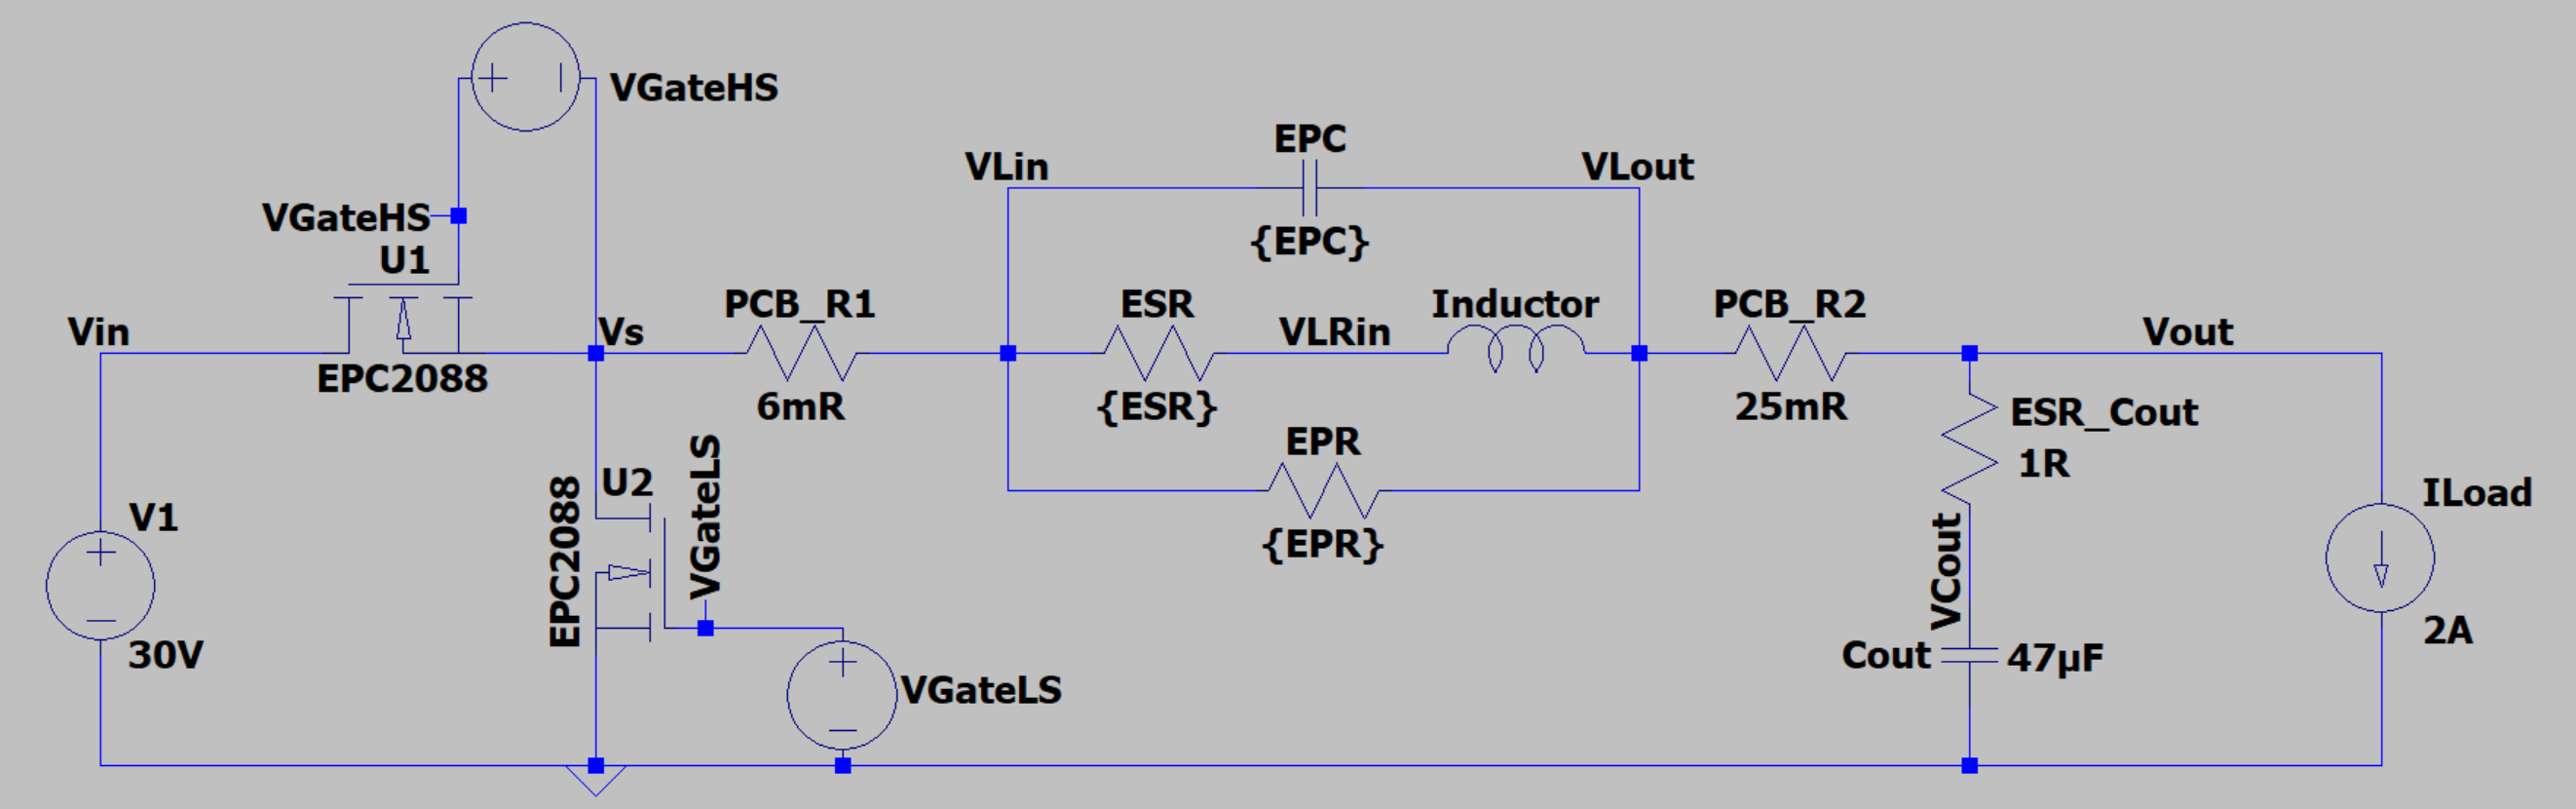
\includegraphics[width=1\linewidth]{Bilder//Kapitel4/BC_LTspice.png}
    \caption{Complete Synchronous Buck Converter in LTspice with the \textit{EPC2088}}
    \label{fig:BC_LTspice}
\end{figure}
Measuring the individual currents, voltages and powers is done via the \textit{.meas}-command, which outputs the average of the observed functions for each given switching frequency and buck converter to an external file. To calculate this average, LTspice simply adds up the values of its output graph, only taking into account the displayed part of the signal. Because of this, it is crucial that always a whole number of periods is displayed, to create an accurate measurement. The buck converter is therefore given a set amount of time to settle after which ten periods are displayed and used for the measurements. 

\subsection{Simulating the Buck Converter}\label{sec:simulating_the_buck_converter}
To compare the results of the simulation with those of the measurement, the different combinations of inductors and \acp{GaNFET} are simulated at the same switching frequencies used in the measurements. The buck converter with the inductor \textit{XGL1313-103ME} is again used to present the different efficiency behaviours of the \acp{GaNFET}. In the following figure, the simulated efficiencies are directly compared to the results of the measurements of section \ref{sec:measuring_the_buck_converter}. 
\begin{figure}[H]
    \begin{subfigure}[b]{0.50\textwidth}
        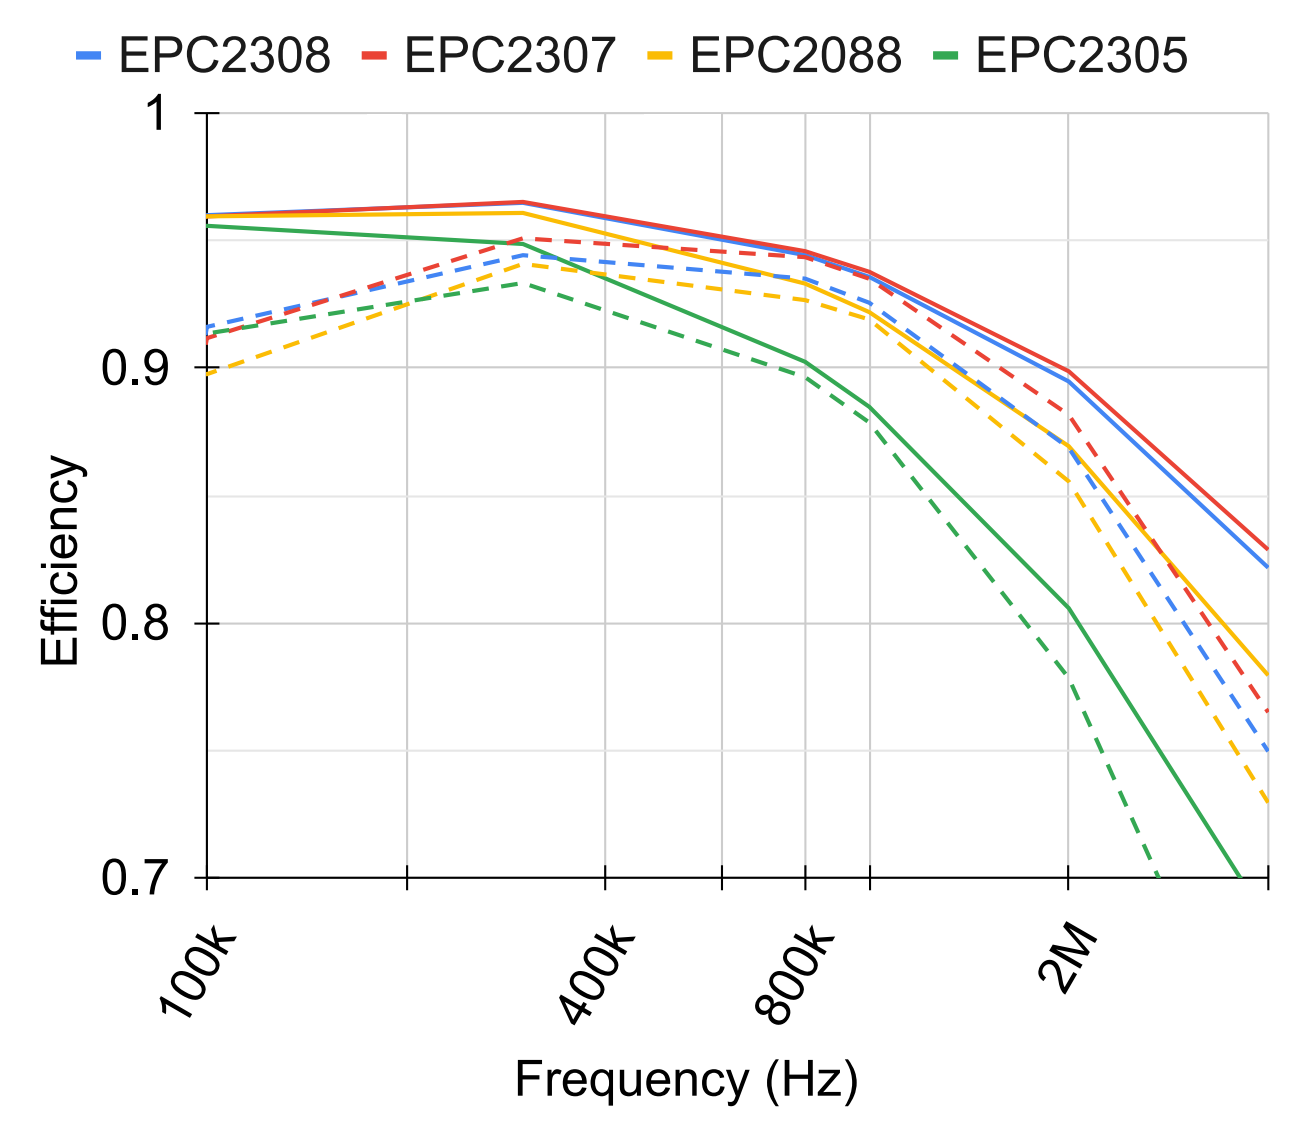
\includegraphics[width=\textwidth]{Bilder/Kapitel4/XGL103 Efficiency Simulated and measured.png}
    \end{subfigure}
    \begin{subfigure}[b]{0.50\textwidth}
        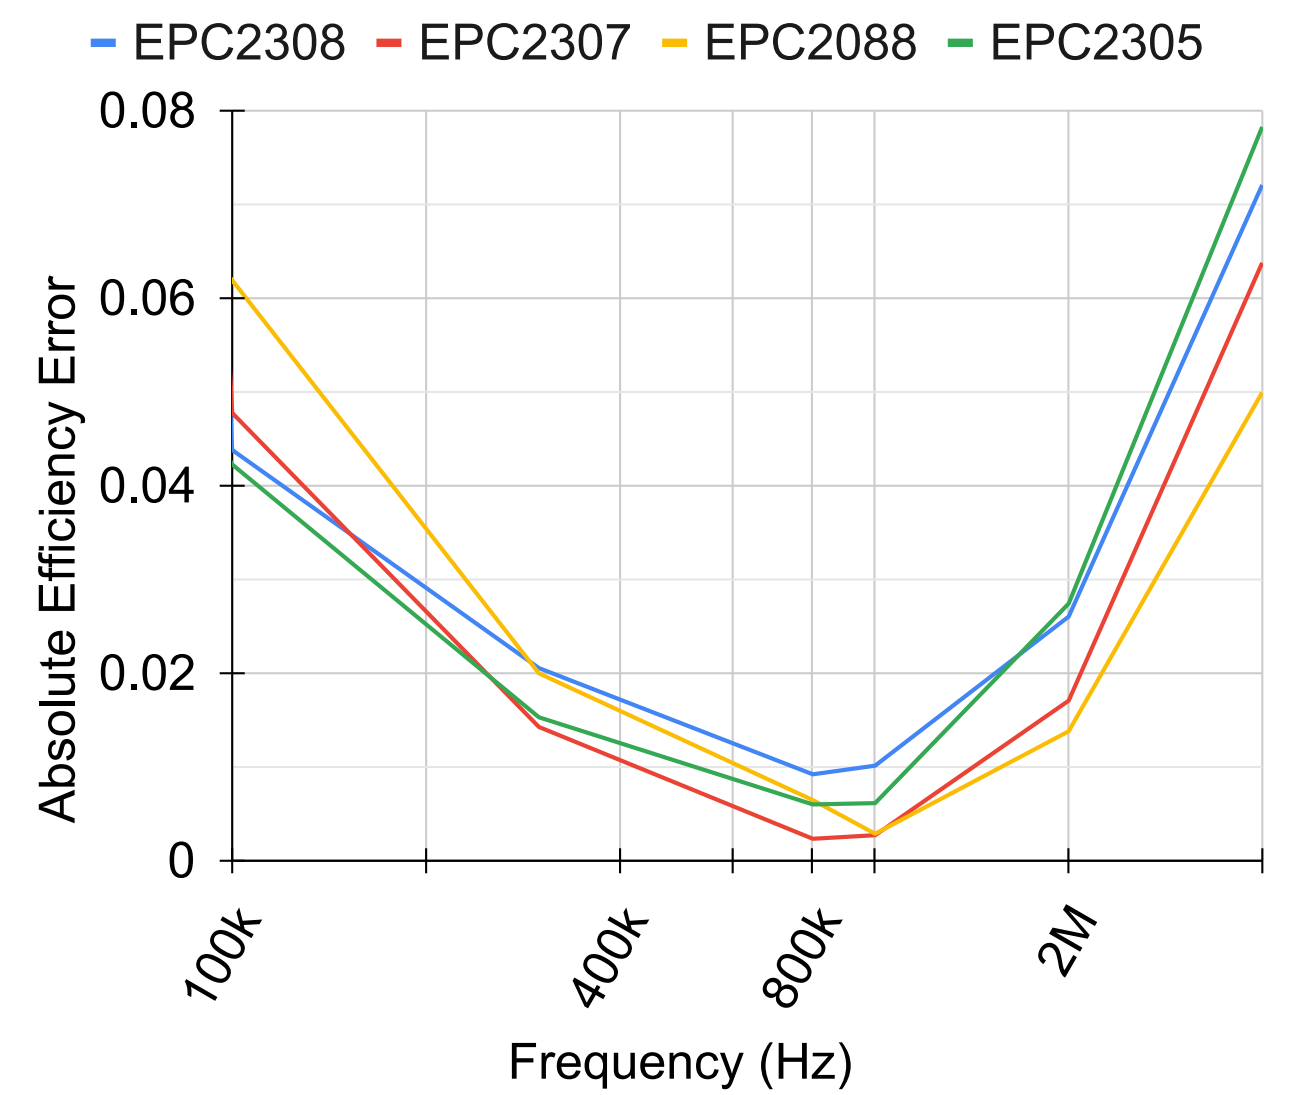
\includegraphics[width=\textwidth]{Bilder/Kapitel4/XGL103 Efficiency Simulated and measured error.png}
    \end{subfigure}
    \caption{Comparison of the simulated and measured buck converter's efficiencies for the \textit{XGL1313-103ME} inductor\\striped lines indicate measured values, while continuous lines are simulated}
    \label{fig:comparison_efficiencies_sim_and_meas}							
\end{figure}
A noticeable error of around 5\% for all Types of \acp{GaNFET} appears at the low end of the frequency range. With increasing frequency the simulation first approaches the measured efficiency, reaching a minimal error of less than 1\% at a switching frequency of \SI{1}{\mega\Hz}, after which the error again increases. Overall the efficiency in the simulation is higher, than the measured efficiency, hinting at physical losses that are not represented in the simulation. Still, the approximate shape of the simulated efficiency curve follows that of the measured efficiency curve.\\
Taking a closer look at the loss distribution of an individual buck converter shown in figure \ref{fig:xgl103_epc2088_loss_comparison}, gives an insight into the missing loss sources. To keep the example used in section \ref{sec:measuring_the_buck_converter}, the buck converter using the \textit{XGL1313-103ME} inductor and the \ac{GaNFET} \textit{EPC2088} is examined. Firstly, the simulation shows a linear rise in the \ac{GaNFET} losses in respect to the switching frequency, showing that the switching losses are represented by the simulation. At low switching frequencies, the model however deviates from the expected behaviour, as the losses in the \ac{GaNFET} are now attributed mainly to effects, other than the switching losses.\\
Similarly, the behaviour of the simulated inductor also strays from the measured behaviour. At low switching frequencies, the simulated inductor losses start out high and begin to decrease as the frequency increases. While this reduction continues on in the measured inductor, it halts for the simulated inductor. The simulated inductor thereby undershoots the losses at low frequencies and overshoots the measured losses at high frequencies.
\begin{figure}[H]
    \centering
    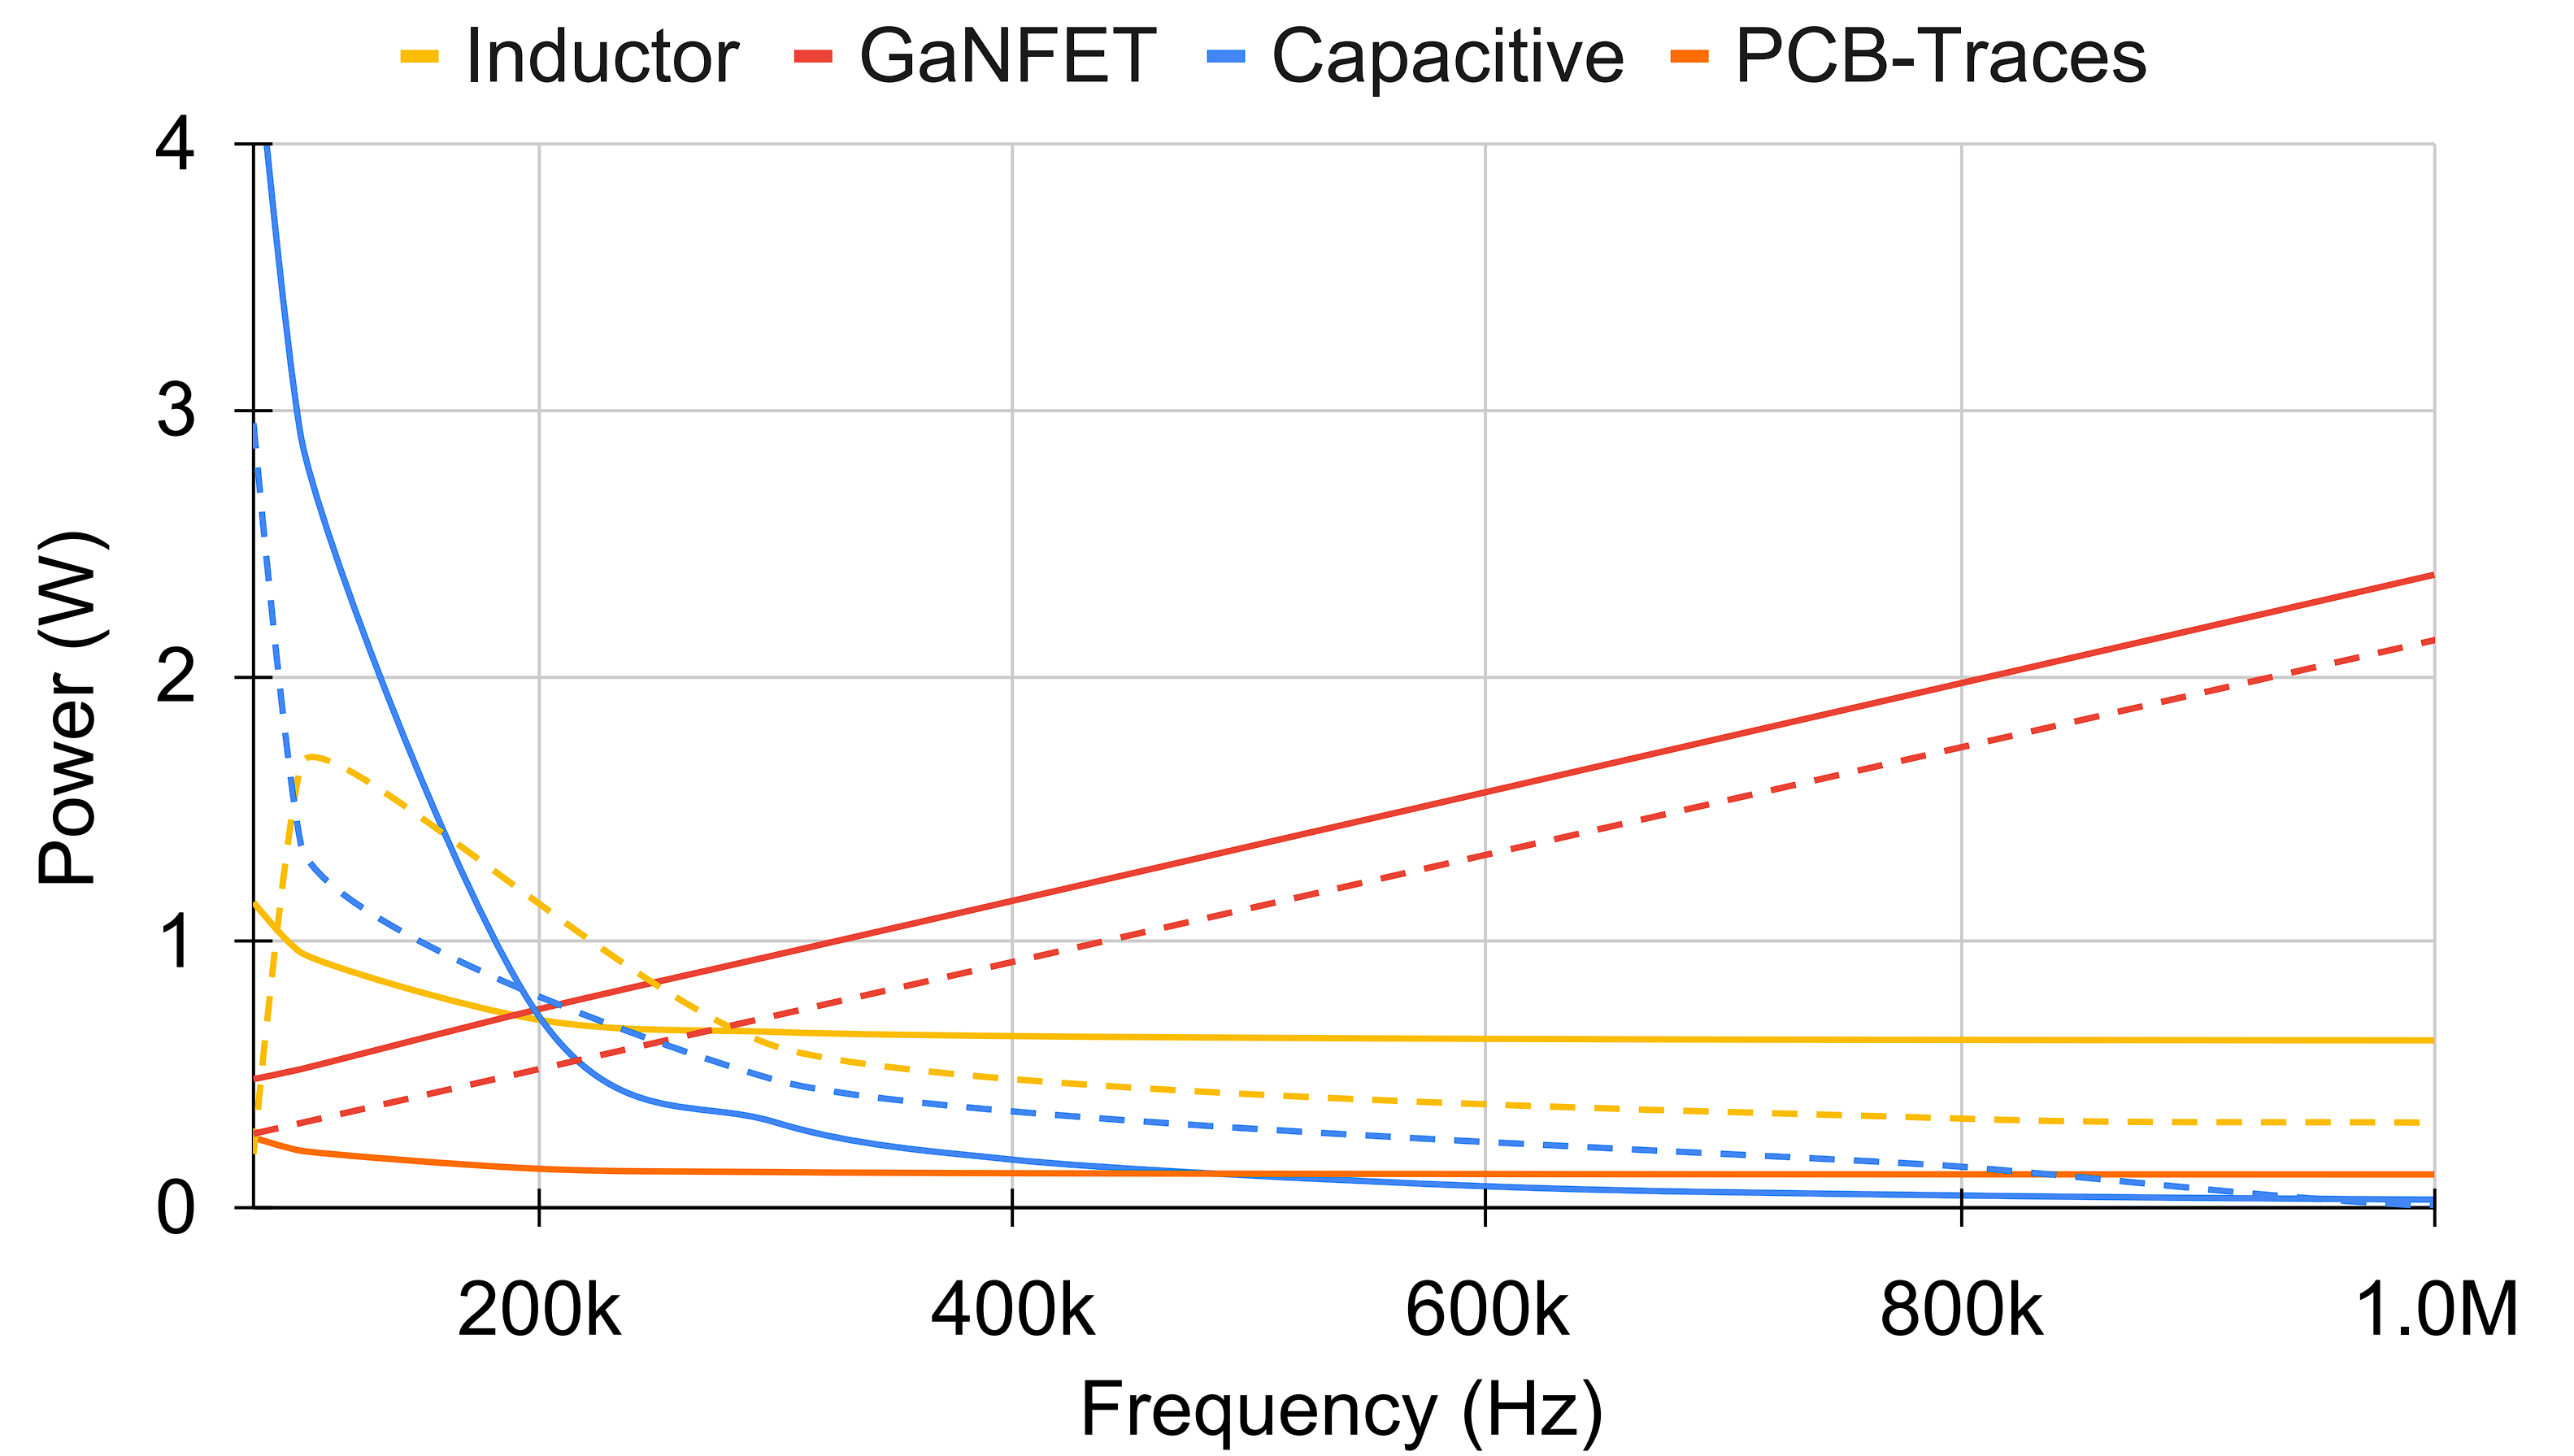
\includegraphics[width=0.75\linewidth]{Bilder/Kapitel4/XGL103_EPC2088_Simulation_Loss_Comparison.png}
    \caption{Comparison of the inductor and switching losses for the buck converter consisting of the \textit{XGL1313-103ME} inductor and \textit{EPC2088} \acp{GaNFET}}
    \label{fig:xgl103_epc2088_loss_comparison}
\end{figure}
Transferring the individual loss behaviour of the simulation back to figure \ref{fig:comparison_efficiencies_sim_and_meas}, shows that this difference in behaviour is not only observed for this specific buck converter but across all four different buck converters with the \textit{XGL1313-103ME} inductor. In fact, this discrepancy between the measured and simulated behaviour holds true for all observed buck converters.

%--> Comparison of the measured and simulated values --> At what frequency is the buck converter optimal? (does this approach the same point, as measured
%--> What are the differences, why is the efficiency so much higher, than in real life?
%--> How big is the error, and is it usable?
 
\section{Evaluation}\label{sec:evaluation}
The results of section \ref{sec:complete_simulation_of_the_buck_converter} show how the behaviour of a given synchronous buck converter can be approximated by LTspice. Incorporating the \ac{ECM} of the used inductor and a fitting model for the switching element, yield loss simulations that approximate the true behaviour and deliver insights about the efficiency characteristics of the observed synchronous buck converter. These simulations however have non-negligible shortcomings. As the sole \ac{ECM} is not able to truly represent the core losses, the losses of the inductor are only a rough approximation of the actually occurring losses. Due to hysteresis and the effect of \ac{DC} bias not being able to be represented by a simple \ac{ECM}, another method is necessary to reduce the error of the simulation. Yet, as shown in section \ref{sec:hysteresis_behaviour_of_the_inductor}, the LTspice inbuilt hysteresis solver is not capable of providing a fitting solution.\\
Apart from the inductor, section \ref{sec:simulating_the_buck_converter} shows that the provided \ac{GaNFET} models also do not behave like their physical counterparts. While their switching losses are well-modelled, the low-frequency losses measured in the buck converter are not represented by the model.\\
Taking these inaccuracies into account, the LTspice model is still able to provide an estimate of the ideal switching frequency for a given synchronous buck converter. Running the simulation for smaller frequency increments shows how the simulation gives bounds in which the ideal switching frequency lays. 
\begin{figure}[H]
    \centering
    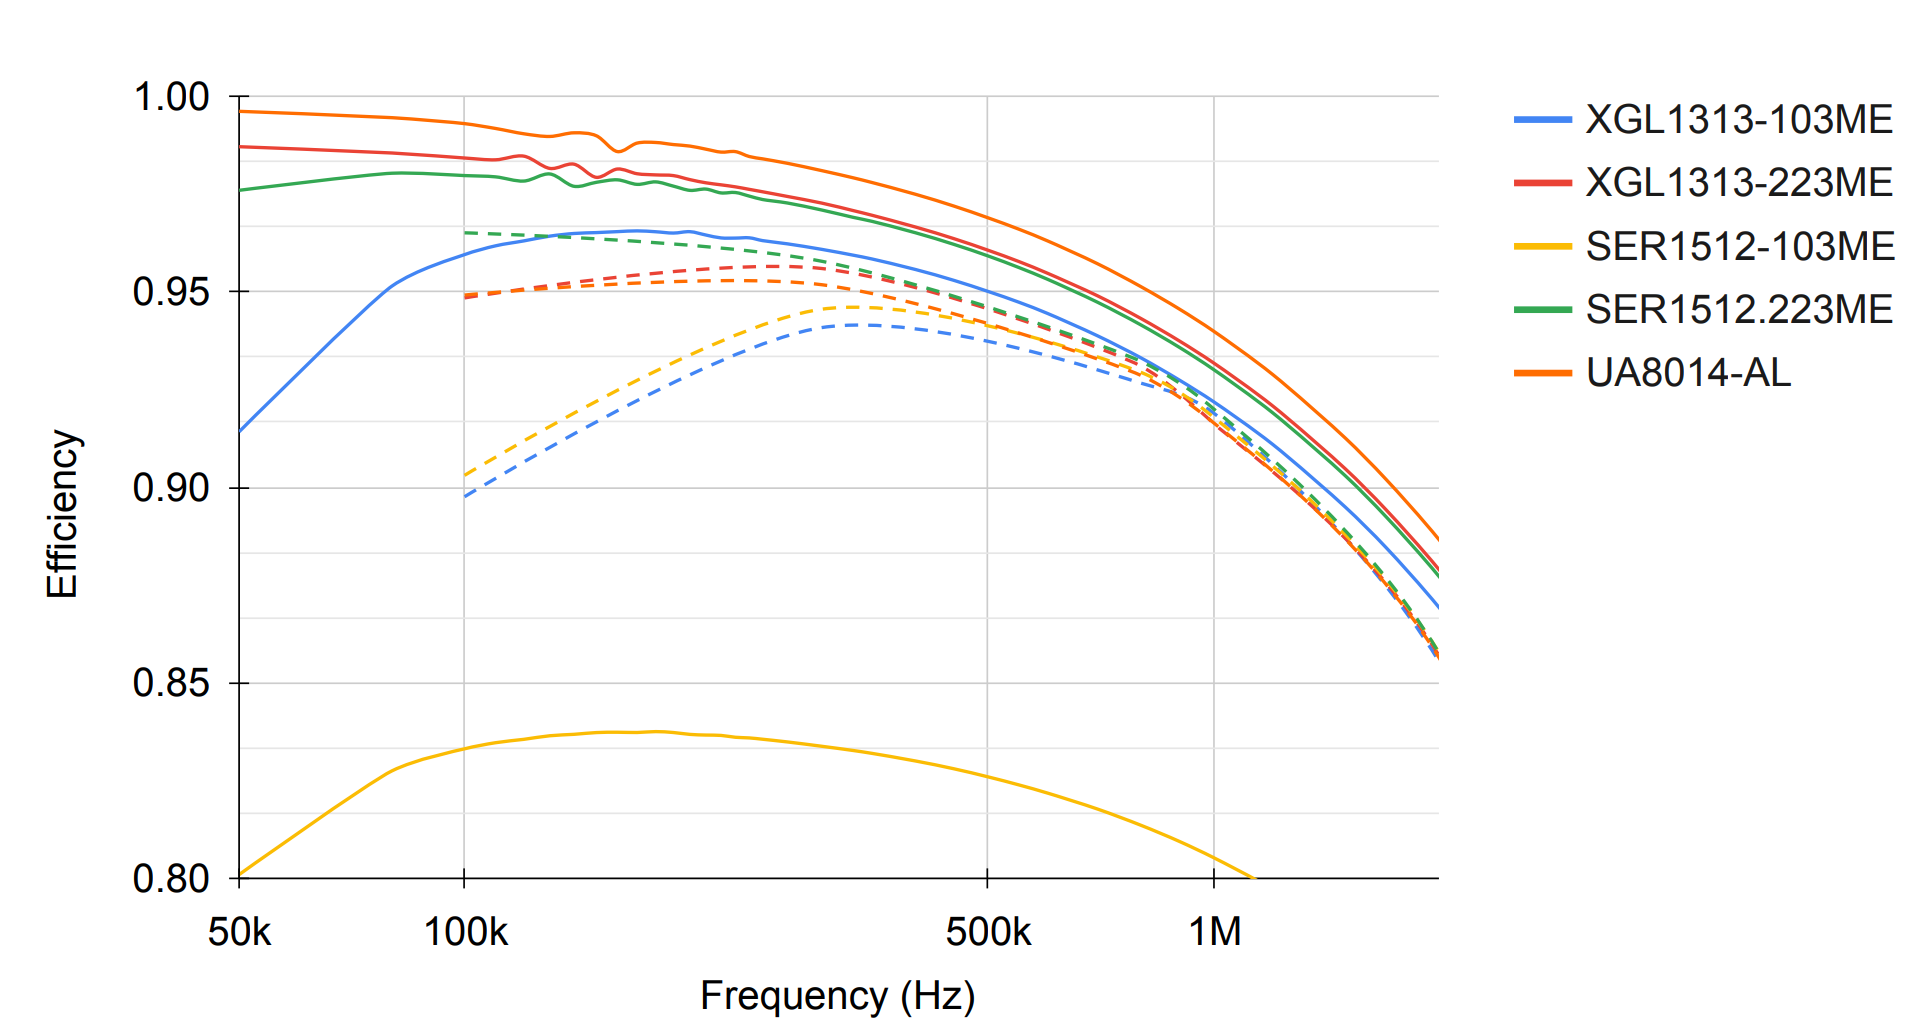
\includegraphics[width=1\linewidth]{Bilder/Kapitel4/Efficiency_Simulation_Comparison.png}
    \caption{Comparison of the simulated and measured efficiency of the different buck converters all using the \textit{EPC2088} \ac{GaNFET} \\striped lines indicate measured values, while continuous lines are simulated}
    \label{fig:efficiency_simuilation_comparison}
\end{figure}
Demonstrated by the buck converter of the \textit{XGL1313-103ME} inductor and \textit{EPC2088} \ac{GaNFET}, the simulation defines a range between \SI{80}{kHz} and \SI{500}{kHz}, where the efficiency is at a maximum. This coincides with the measurement, which predicts an ideal switching frequency of \SI{300}{kHz}. Hence, this estimation can then be used to determine the true ideal switching frequency through real-world measurements. 



%--> Is this method feasible, does it help? Where are the limitations?
%\todo[inline]{Validate the inductor ECM}
%\todo[inline]{Validate the saturation model}
%\todo[inline]{Explain the Buck Converter Measurement Setup, in the lab and in LTspice}
%\todo[inline]{Compare the losses of both measurments}

%\todo[inline]{Evaluate the accuracy}
%\todo[inline]{Explain the short commings of the work --> Show the error}
%\todo[inline]{Goal --> Repeatability has to be reservered (all necessary data to repeat the experiments needs to be mentioned)}
